\documentclass{article}
\usepackage{url}
\usepackage{graphicx}
\graphicspath{ {./source/images/} }

\begin{document}

  \section{Introduction to Twisted}
    [ADD Examples of Twisted]

  \section{Event-driven Programming paradigm}
    \subsection{Single thread}
      Single threaded or sequential programming is in which requests are
      processed by a single thread. If the thread is doing some blocking task
      like IO then the program can't handle any other requests until the
      request is processed.

      Example of single threaded server
      \begin{verbatim}
        import time

        from http import server
        from socketserver import ThreadingMixIn


        class RequestHandler(server.SimpleHTTPRequestHandler):

            def do_GET(self):
                start_time = time.time()
                time.sleep(5)
                end_time = time.time()
                self.send_response(200, "OK")
                self.end_headers()
                response = (
                    "Started at {}, Ended at {} difference {}".format(
                        start_time, end_time, end_time - start_time
                    )
                )
                self.wfile.write(response.encode('utf-8'))
                return

        with server.HTTPServer(
          ('localhost', 8000), RequestHandler
        ) as http_server:
            http_server.serve_forever()
      \end{verbatim}

    \subsection{Multi-Threaded}
      Converting above program to a multithreaded version will help. A
      multithreaded program will handle each HTTP request in a new thread and
      thus it can handle mutiple requests at the same time.

      \begin{verbatim}
        import time

        from http import server
        from socketserver import ThreadingMixIn


        class RequestHandler(server.SimpleHTTPRequestHandler):

            def do_GET(self):
                time.sleep(40)
                end_time = time.time()
                self.send_response(200, "OK")
                self.end_headers()
                response = "Ended at {}".format(end_time)
                self.wfile.write(response.encode('utf-8'))
                return


        class ThreadedHTTPServer(ThreadingMixIn, server.HTTPServer):
            daemon_threads = True


        with ThreadedHTTPServer(
            ('localhost', 8000), RequestHandler
        ) as http_server:
            http_server.serve_forever()
      \end{verbatim}

      Compared to the single threaded approach, the program with multithreaded
      will be able to achieve more performance because the server will spawn a
      new thread for each new request. And thus, when the thread is blocking,
      it can handle another request during that time.

      But here is a problem. When bunch of new requests are coming (usually
      higher than the core of processor), Blocking thread is actually blocking
      the CPU core.

      Compare the threaded example using Apache Benchmark tool.

      \begin{verbatim}
        ab -n 100 -c 100 -s 120 http://localhost:8000
      \end{verbatim}

      In the above, command \textbf{-n} is a short-hand for Number of requests
      to be fired. \textbf{-c} is a concurrent requests the tool will fire at
      the same time. \textbf{-s} is a short hand for total number of seconds
      after which the tool will timeout a request.

      The threaded server, a maximum number of concurrent requests handled by
      the server will be somewhere between (total number of cores * 1.5 ) + 1.
      The server can't handle other concurrent requests at the same time. The
      server will process those requests in batches.

    \subsection{Event-driven}
      Now, if we convert above example into event-driven asynchronous code
      then it will look as below.

      \begin{verbatim}
        import time

        from twisted.internet import reactor
        from twisted.internet.task import deferLater
        from twisted.web.resource import Resource
        from twisted.web.server import Site, NOT_DONE_YET


        class BusyPage(Resource):
            isLeaf = True

            def _delayedResponse(self, request):
                end_time = time.time()
                response = "Ended at {}".format(end_time)
                request.write(response.encode("utf-8"))
                request.finish()

            def render_GET(self, request):
                d = deferLater(reactor, 40, lambda: request)
                d.addCallback(self._delayedResponse)
                return NOT_DONE_YET


        factory = Site(BusyPage())
        reactor.listenTCP(8000, factory)
        reactor.run()
      \end{verbatim}

    Compare the performance of the above code by Apache benchmarking tool.

    Below is the same command we had used earlier to compare the multi-threaded
    approach.

    \begin{verbatim}
      ab -n 100 -c 100 -s 120 http://localhost:8000
    \end{verbatim}

    The output statistics of both the command will be different. The
    asynchronous approach will be able to handle all the requests at the same
    time. Reason behind this is when the request is coming, the IO thread is
    trying to process the request. During that time, if it is blocked the code
    is handled by event-driven approach and the thread is again available for
    entertaining another request. The processing of request is again resumed
    when the duration of IO is completed and returned.

    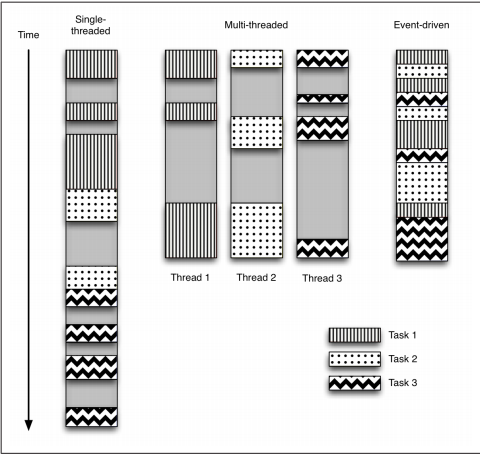
\includegraphics{event_driven_comparision.png}

  \section{Introduction to Twisted programming}

    \subsection{History}
      Twisted was invented by \texttt{Glyph Lefkowitz} in the year October 22,
      2002 which is almost 16 years before. It is an old giant.

    \subsection{Current situation}
      At present, the Twisted framework is developed and managed by its
      community. Latest stable version is \textbf{18.9.x}. The Twisted
      framework is licensed under MIT license. Twisted is based on event-driven
      programming paradigm.

    \subsection{Sockets}
      Twisted programming supports all the TCP, UDP, SSL/TSL based sockets. It
      also supports the Unix sockets.

    \subsection{Protocol}
      Twisted supports many application layer protocols. Such as HTTP, XMPP,
      IMAP, SSH, IRC, FTP and many more.

    \subsection{Applications/Frameworks based on Twisted}

    \begin{iteritems}
      \item Buildbot
      \item Omgle video chat service
      \item Twilio a cloud telephony provider
      \item Twitch.tv a popular Game livestream video sharing
      \item Scrapy a framework for scrapping webpages
    \end{iteritems}

  \section{Reactor}
    Reactor is the core of the event loop. It is responsible for waiting for
    the event and notify the program when the event is occurred. Reactor is
    dependent on platform specific libraries. Twisted will automatically choose
    default platform specific library.

    For under the hood details, In GNU/Linux platform it tries to fetch for
    epoll \cite{epoll}.  If epoll \cite{epoll} is not available, it will use
    poll \cite{poll}. All the POSIX compliant platforms it will use poll. All
    other platforms such as Windows and Macintosh it will use select reactor.

    You have to register your callbacks to the reactor and have to start it.
    Once the reactor is start, it will listen to the events and notifies to the
    program forever or until \texttt{reactor.stop} is called.

    \begin{verbatim}
      // Example reactor_server.py
      from twisted.internet import reactor

      reactor.listenTCP(8000, MyFactory())
      reactor.run()
    \end{verbatim}

  \section{Transport}

    Transport is responsible to provide the behaviour for transferring data to
    the other end of the connection. The transport behaves differently
    according to the connection for example, TCP or UDP will have different
    implementation of transport. All the transport implementations should be
    dependent on \texttt{ITransport} interface.

    Common methods are

    \subsection{write} Should write data to the connection.

    \subsection {writeSequence} Should write list of strings to the connection.

    \subsection{loseConnection} Should close the connection after writing
    ending data.

    \subsection{getPeer} Should return remote address of the connection.

  \section{Protocol}
    Protocol will define the behaviour to process the network events in async
    manner. Twisted does have in-built definition for many protocols such as
    HTTP, Telnet, DNS etc. All the protocol classes should implement
    \texttt{IProtocol} interface. Base class is \texttt{protocol.Protocol}.

    Common methods are

    \subsection{makeConnection} Should create a connection.

    \subsection{connectionMade} Should be called when a new connection is made.

    \subsection{dataReceived} Should be called when any data is received from
    the other end of the circuit.

    \subsection{connectionLost} Should be called when the connection is
    terminated.

  \section{Protocol Factory}
    The factory will produce the instance of \texttt{Protocol} when the new
    connection is made. \texttt{Protocol} will be garbage collected when the
    collection is called. The Factory will store configuration details for
    \texttt{Protocol} instances. The factory is following
    \texttt{IProtocolFactory} interface. There client implementation of common
    factory methods is \texttt{ClientFactory}.

    Methods

    \subsection{buildProtocol} should create the instance of Protocol class.

  \begin{thebibliography}{2}
    \bibitem{epoll}
      \url{http://man7.org/linux/man-pages/man7/epoll.7.html}% chktex 8
    \bibitem{poll}
      \url{http://man7.org/linux/man-pages/man2/poll.2.html}% chktex 8
    \bibeitem{buildbot}
      \url{https://buildbot.net/} % 

  \end{thebibliography}
\end{document}
